% file: h-layout-2.tex
% url: https://tex.stackexchange.com/q/145116/23098

\documentclass[tikz]{standalone}
\tikzset{if/.code n args={3}{\pgfmathparse{#1}%
  \ifnum\pgfmathresult=1\pgfkeysalso{#2}\else\pgfkeysalso{#3}\fi}}

\begin{document}
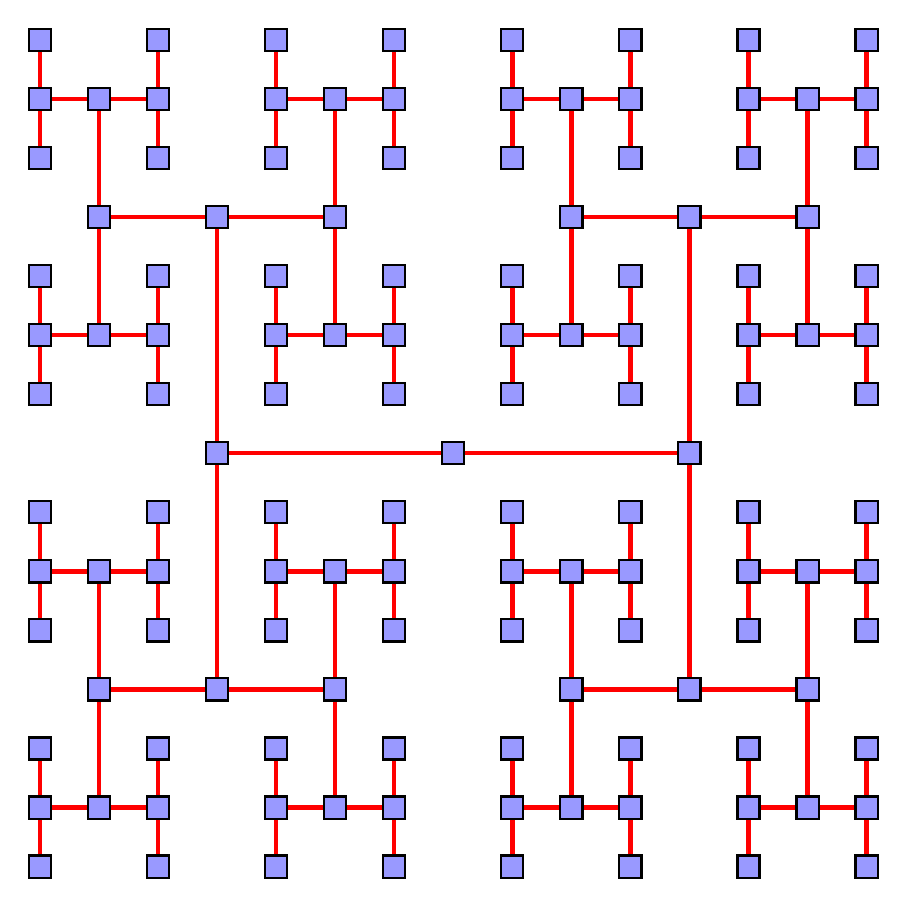
\begin{tikzpicture}[nodes=draw, thick,
    every node/.style = {draw, rectangle, inner sep = 4pt, fill = blue!40},
    every edge/.style = {draw, red, ultra thick},
  H/.style n args={3}{% #1 = direction, #2=initial length, #3=levels
    if={0<=#3}{
      append after command={\pgfextra{\let\tikzLastnode\tikzlastnode}
        node[HH={#1}{#2}{#3}, shift=(#1+180:#2)] at (\tikzLastnode) {} edge (\tikzLastnode)
        node[HH={#1}{#2}{#3}, shift=(#1:#2)]     at (\tikzLastnode) {} edge (\tikzLastnode)}
    }{}},
  HH/.style n args={3}{
    append after command={\pgfextra{\let\tikzLastnode\tikzlastnode}
      node[H={#1}{#2/2}{#3-1}, shift=(#1+90:#2)] at (\tikzLastnode) {} edge (\tikzLastnode)
      node[H={#1}{#2/2}{#3-1}, shift=(#1-90:#2)] at (\tikzLastnode) {} edge (\tikzLastnode)
    }}]
\node[H={0}{3cm}{2}] {};
\end{tikzpicture}
\end{document}
